\documentclass{article}
\usepackage{fullpage}

\usepackage{epsfig}
\usepackage{amsfonts}
\usepackage{amssymb}
\usepackage{amstext}
\usepackage{amscd}
\usepackage{amsmath}
\usepackage{amsthm}
\usepackage{times}
\usepackage{graphicx}
\usepackage{alltt}
\usepackage{algpseudocode}

\begin{document}

%\thispagestyle{empty}

\noindent
\fbox{
\parbox{\textwidth}{
\begin{Large}
{\bf CS 577: Introduction to Algorithms\hfill Dynamic Program Review}
\end{Large}
}}

\subsection*{Problems}

\begin{enumerate}
\item During thanksgiving break Alice is planning to make a road trip from Madison to Seattle, and wants to stop at various tourist locations along the way for sight-seeing. The locations are numbered from 1 through $n$
with $n$ being Seattle, and this is the order that Alice wants to visit them in. Furthermore, since she has a limited amount of time for the trip, she wants to spend no more than $x$ hours driving.

Your goal is to help Alice plan her trip. You are given a directed
graph over locations with each edge between two locations specifying
the amount of time it takes to drive from one to the other. Design an
algorithm that returns a path from Madison to Seattle with total
driving time $\le x$ hours, and that visits the maximum possible number of locations enroute. Your algorithm should run in time polynomial in the size of the graph (number of vertices and edges), independent of $x$. An algorithm running in time polynomial in the size of the graph as well as $x$ will receive partial credit.

\begin{center}
	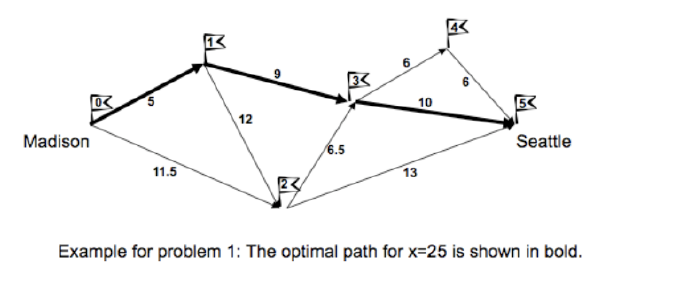
\includegraphics[width=100mm]{graph.png}
\end{center}

\item In class, we developed an $O(nW)$ time algorithm for the
  Knapsack problem, where $n$ is the number of items and $W$ is the
  capacity of the knapsack. Recall that in this problem our goal is to
  fill the knapsack with items whose weights add up to no more than
  $W$ and whose total value is maximized. Each item can only be picked
  once.

  Suppose that the capacity $W$ is very large (say, exponential in
  $n$), so that the running time $O(nW)$ is prohibitively
  large. Suppose further that each item has a small integral
  value. Design a different dynamic program for this problem that runs
  in $O(nV)$ time, (that is, a running time independent of $W$,) where
  $V=\sum_i v_i$ is the sum of values of all the items. You may assume
  that integer operations take $O(1)$ time. Give a brief argument of
  correctness and an analysis of the running time of your algorithm.

  (Hint: you will need to modify the recursive definition we used to
  construct the $O(nW)$ time algorithm.)
  
 \item You are given an array $A$ of $n$ numbers, each of which may be positive, negative, or zero. Your goal is to find a contiguous subarray $A[i, \cdots, j]$ such that the sum of its elements $A[i], \cdots , A[j]$ is maximized.

For example, for the array $[4, -11, 9, 3, -2, 10, -5, 1, 2]$, the subarray $[9, 3, -2, 10]$ achieves the maximum sum, 20.

Develop a recursive algorithm that finds the maximum sum in a contiguous subarray. Memoize it to obtain a dynamic program. Analyze its running time. (Your DP should run in $O(n)$ time.)

\item You are in charge of planning the bus route for a single bus for your local school district. The school and all of the bus stops on the route are located at exits along an east-west highway, and the bus route begins at the school. Think of the highway as a straight line with the school somewhere in the middle. You know how many students will get off of the bus at each exit. The bus may drive along the highway in either direction, switching directions as often as necessary. Your goal is to design a route such that the sum over the children of the total distance each child travels is minimized. 

For example, suppose there are two bus stops, one at a distance of 1 from the school in one direction along the highway with 2 children getting off, and the other at a distance of 2 in the other direction with 5 children getting off. If the bus route goes to the first stop and then the second, the total distance traveled by the kids is $1 \times 2  + (1 + 1 + 2)\times 5 = 22$. If the bus route goes to the second stop and then to the first, the total distance
traveled is $2 \times 5 + (2 + 2 + 1) \times 2 = 20$. So the second route is preferable.

Design a dynamic program to output the optimal bus route. Your input consists of a sorted list $L$ of size n, where $L[i]$ specifies the distance of the $i$th exit from the east-most exit (so, in particular, the first distance in the list is 0). You are also given the location of the school, again in the form of its distance from the east-most exit.
Finally, you are given a list $S$ of size $n$, where $S[i]$ specifies the number of students to be dropped off at the $i$th exit in east to west order. Your algorithm should run in time polynomial in the number of exits.

\item You are given an arithmetic expression containing $n$ integers and $n - 1$ operators, each either $+$, $-$, or $\times$. Your goal is to perform the operations in an order that maximizes the value of the expression. Your function should output this maximum value.

For example:
\begin{itemize}
\item For the expression $6\times 3 + 2 \times 5$,the optimal ordering is to add the middle numbers first, then perform the multiplications: $((6 \times (3 + 2)) \times 5) = 150$.
\item For the expression $(-3) \times 3 + 3$, the optimal ordering is $(((-3) \times 3) + 3) = -6$. 
\item For the expression $(-3) \times 3 - 3$, the optimal ordering is $((-3) \times (3 - 3)) = 0$.
\end{itemize}


\item
A \textbf{supersequence} of a sequence is obtained by adding elements to the given sequence (in any locations). For example, dynamicprogramming is a supersequence of the sequence damn. A \textbf{palindrome} is a sequence which reads the same backwards and forwards. For example, amanaplanacanalpanama is a palindrome.
In this problem you are given a sequence A of length n and your goal is to find the shortest supersequence of $A$ that is a palindrome. Develop a recursive algorithm for this problem. Memorize it to obtain a dynamic program. Analyze its running time. (Your DP should run in $O(n^2)$ time.)

\item Martian currency has n different coins with integral denominations $a_1 \cdots a_n$. For a given integer value $A$, your goal is to make change for a total amount of $A$ using the fewest number of coins possible. Your function should return the fewest number of coins needed to make change.


\item \textit{Gerrymandering} is the practice of carving up electoral districts in very careful ways so as to lead to outcomes that favor a particular political party. Recent court challenges to the practice have argued that through this calculated redistricting, large numbers of voters are being effectively
(and intentionally) disenfranchised.

Suppose we have a set of $n$ precincts $P_1, P_2, \cdots, P_n$, each containing $m$ registered voters. We're supposed to divide these precincts into two districts, each consisting of $n/2$ of the precincts. Now, for each precinct, we have information on how many voters are registered to each of two
political parties. (Suppose, for simplicity, that every voter is registered to one of these two.) We'll say that the set of precincts is \textit{susceptible} to
gerrymandering if it is possible to perform the division into two districts in such a way that the same party holds a majority in both districts.

Give an algorithm to determine whether a given set of precincts is susceptible to gerrymandering; the running time of your algorithm
should be polynomial in $n$ and $m$. 

\textbf{Example}. Suppose we have $n = 4$ precincts, and the following information
on registered voters.

\begin{center}
  \begin{tabular}{ l | c | c | c | c }
    \hline
    Precinct & 1 & 2 & 3 & 4\\ \hline
    Number registered for party A & 55 & 43 & 60 & 47 \\ \hline
    Number registered for party B & 45 & 57 & 40 & 53 \\
    \hline
  \end{tabular}
\end{center}


This set of precincts is susceptible since, if we grouped precincts 1 and 4 into one district, and precincts 2 and 3 into the other, then party
A would have a majority in both districts. (Presumably, the ``we" who are doing the grouping here are members of party A.) This example is a quick illustration of the basic unfairness in gerrymandering: Although party A holds only a slim majority in the overall population (205 to 195), it ends up with a majority in not one but both districts.

\bigskip

\end{enumerate}

\end{document}